% ------------------------------------------------------------------------------
% --------------------------------- Question 1 ---------------------------------
% ------------------------------------------------------------------------------
\subsection{Question 1}

The result of the initialization of the clustering process depends on whether
there is a priori knowledge about the image to be segmented. In this example,
where image ``orange" is known, we can specify the colour of each initial
cluster depending on what the image's dominant colours are. In this case where
the colour diversity is low, it is possible to set two initial kernel values
to the colours ``orange" (roughly $(255,150,0)$ in the image in question)
and ``white" (exactly $(255,255,255)$ in the image in question)
and let the rest of the kernels be chosen in random,
to the extent of what level of detail is desirable.

In general, where the image to be segmented and its context may be unknown,
the best way to initialize the kernels, so as to achieve a result that is not
wrongly biased, is to let them be chosen at random, optinally with provision
having been taken regarding the diversity of initial colours.

Figures \ref{fig:orange}, \ref{fig:orange_segmented}
and \ref{fig:orange_segmented_bounds} illustrate the k-means segmentation
method for image \texttt{orange} with
\texttt{(K,L,scale\_factor, $\sigma$) $\equiv$ (8,10, 1, 1)}.


\begin{figure}[H]
	\centering
  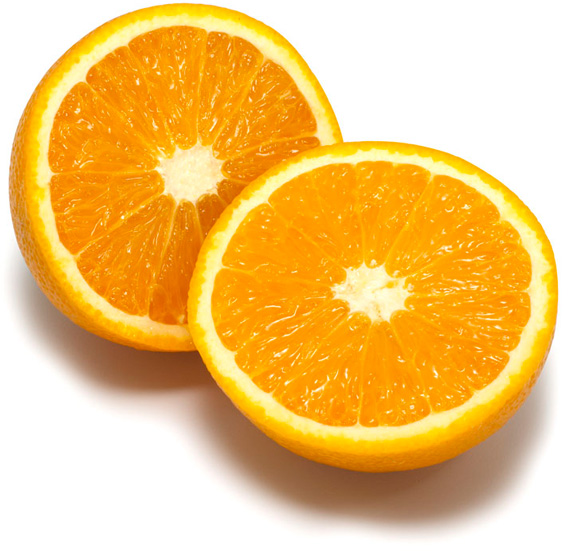
\includegraphics[scale=0.4]{../../bildat_lab3/orange.jpg}
  \caption{The original image.}
  \label{fig:orange}
\end{figure}

\begin{figure}[H]
	\centering
  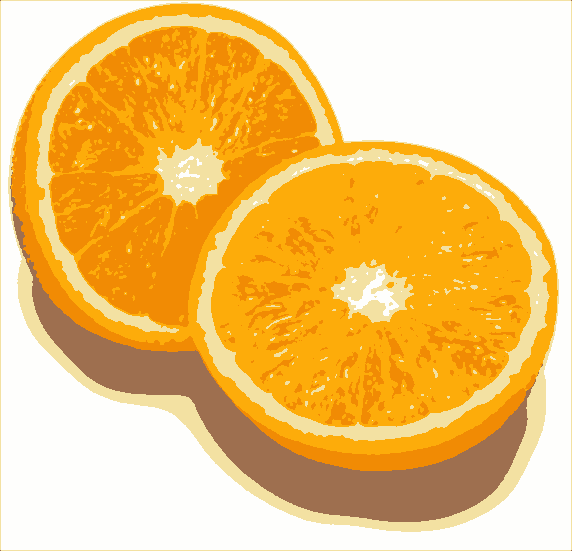
\includegraphics[scale=0.4]{./images/01/default1.png}
  \caption{The image segmented.}
	\label{fig:orange_segmented}
\end{figure}

\begin{figure}[H]
	\centering
  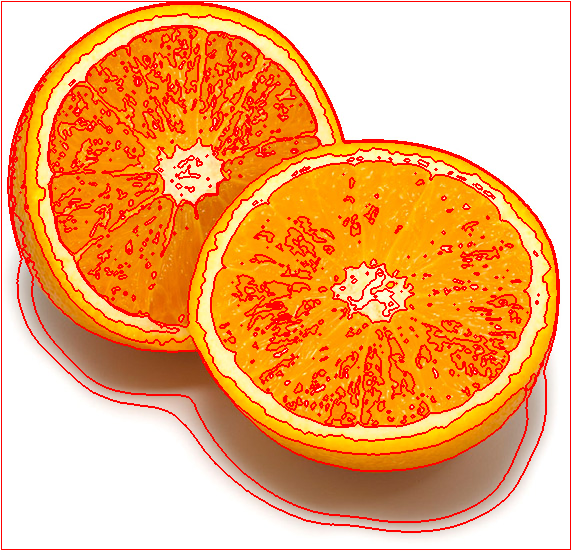
\includegraphics[scale=0.4]{./images/01/default2.png}
  \caption{The image and the bounds of its segments.}
  \label{fig:orange_segmented_bounds}
\end{figure}


% ------------------------------------------------------------------------------
% --------------------------------- Question 2 ---------------------------------
% ------------------------------------------------------------------------------
\subsection{Question 2}
Convergence time depends linearly on the number of clusters $K$ chosen.
Furthermore it depends on the colour diversity of the image.
Tables \ref{tab:convergence_orange} and \ref{tab:convergence_tiger} illustrate
the number of iterations it takes for the k-means clustering method to
reach convergence depending on the number of clusters.

\begin{table}[H]
\centering
\makebox[0pt][c]{\parbox{\textwidth}{%
  \begin{minipage}[b]{0.45\hsize}\centering
    \begin{tabular}{c|c}
    $K$ & convergence iteration \\ \hline
    1                 & 2                     \\
    2                 & 9                     \\
    3                 & 14                    \\
    4                 & 11                    \\
    5                 & 18                    \\
    6                 & 21                    \\
    7                 & 17                    \\
    8                 & 35                    \\
    9                 & 46                    \\
    10                & 23                    \\
    11                & 38                    \\
    12                & 31                    \\
    \end{tabular}
    \caption{Number of centers $K$ and number of iterations taken to reach
      convergence with regard to image \texttt{orange}.}
    \label{tab:convergence_orange}
  \end{minipage}
  \hfill
  \begin{minipage}[b]{0.45\hsize}\centering
    \begin{tabular}{c|c}
      $K$ & convergence iteration \\ \hline
      1                 & 2                     \\
      2                 & 12                    \\
      3                 & 31                    \\
      4                 & 83                    \\
      5                 & 67                    \\
      6                 & 52                    \\
      7                 & 57                    \\
      8                 & 208                   \\
      9                 & 90                    \\
      10                & 103                   \\
      11                & 124                   \\
      12                & 132                   \\
    \end{tabular}
    \caption{Number of centers $K$ and number of iterations taken to reach
      convergence with regard to image \texttt{tiger1}.}
    \label{tab:convergence_tiger}
  \end{minipage}
}}
\end{table}


% ------------------------------------------------------------------------------
% --------------------------------- Question 3 ---------------------------------
% ------------------------------------------------------------------------------
\subsection{Question 3}

% ------------------------------------------------------------------------------
% --------------------------------- Question 4 ---------------------------------
% ------------------------------------------------------------------------------
\subsection{Question 4}
